
\section{Reference Design Expected Performance}
\label{sec:detectors-fd-ref-perf}

The physics requirements are described in \volphys,
for the long-baseline oscillation, atmospheric, supernova
and nucleon decay physics programs.  This section outlines the
numerical detector performance parameters needed to meet the
requirements and the ability of the far detector reference design
to achieve these performance parameters.  

The expected performance of the far detector reference design is based
on the measured performance of the ICARUS\cite{Amerio:2004ze} and
ArgoNeuT\cite{Anderson:2012vc} detectors, scanned Monte Carlo
events\cite{docdb-6954} and newer studies with automated
reconstruction, which are described in
Sections~\ref{sec:detectors-sc-physics-software-simulation-fd},~\ref{sec:detectors-sc-physics-software-reconstruction-fd}
and in \anxreco.  Simulation and reconstruction studies are ongoing.
While many components are in place, a full end-to-end simulation,
reconstruction and analysis chain does not yet exist. Many of the
numerical detector performance requirements are estimates; some of
them correspond to achievements by ICARUS and ArgoNeuT, although these
detectors differ somewhat from the DUNE far detector.  Additional
parameters will be calibrated using the data from LArIAT and the two
CERN prototypes, the \cernsingleproto{} and the \cerndualproto.

Table~\ref{tab:TPC-metric} lists the required performance values,
achieved values (if any) and the values expected from DUNE. The rest
of this section describes each parameter and its connection to the
detector design and physics goals.
\begin{cdrtable}[Preliminary far detector performance expectations]{llll}{TPC-metric}{Preliminary summary of the most 
important performance parameters of the DUNE reference design far
detector.  For each parameter, the table lists the required
(reference) performance, performance achieved by other detectors and
projected performance for DUNE. References are given.  Notes: $^1$For
a MIP at the CPA, minimum in all three views, for any track angle;
$^2$Achieved for the collection view; $^3$In order for the fiducial
volume to be known to $\pm 1\%$, the resolution performances are
reported separately in the $x$, $y$, and $z$ directions, where $z$
points along the neutrino beam axis; $^4$For a sample of stopping
muons; $^5$For electron stubs with $E>5$~MeV.  }
%The third argument (reads {cc}) can use c, l, r or p{some length}  e.g. {clll} or {llp{3cm}}, for instance.
Parameter & Reference Performance & Achieved Elsewhere & Expected Performance \\ \toprowrule
Signal/Noise Ratio$^1$ & 9:1 & 10:1~\cite{Antonello:2015zea,Antonello:2014eha}$^2$ & 9:1 \\ \colhline
Electron Lifetime & 3~ms & $>15$~ms~\cite{Antonello:2014eha} & $>3$~ms \\ \colhline
Uncertainty on Charge & & & \\
Loss due to Lifetime  &   $<1\%$  & $<1\%$~\cite{Antonello:2014eha} & $<1\%$ \\ \colhline
Dynamic Range of Hit & & & \\
Charge Measurement & 15 MIP & & 15 MIP \\ \colhline
% two-hit resolution needs more study.  And likely a different resolution along the drift axis than in the other two directions
% Two-Hit Resolution & 2~mm & & 2~mm \\ \colhline
% Track-finding efficiency is expected to be high.  Needs study to connect it to physics performance
%Track-Finding Efficiency\footnote{For tracks with $L>5$~cm} & $>98\%$ & & $>98\%$ \\ \colhline
Vertex Position Resolution$^3$ & (2.5,2.5,2.5)~cm & & (1.1,1.4,1.7)~cm~\cite{Marshall:2013bda,Marshall:2012hh}\\ \colhline
$e-\gamma$ separation $\epsilon_e$ & 0.9 & & 0.9 \\ \colhline
$e-\gamma$ separation $\gamma$ rejection & 0.99 & & 0.99 \\ \colhline
Multiple Scattering Resolution & & & \\
on muon momentum$^4$ & $\sim$18\% & $\sim$18\%~\cite{gibinmuon,Ankowski:2006ts} & $\sim$18\% \\ \colhline
% electron energy scale uncertainty requirement from LBNE DocDB 8741
Electron Energy Scale & & & From LArIAT \\
Uncertainty & 5\% & 2.2\%\cite{ICARUS-pizero} &  and CERN Prototype \\ \colhline
Electron Energy Resolution & $0.15/\sqrt{E{\rm (MeV)}}$ &$0.33/\sqrt{E{\rm (MeV)}}$  \cite{ICARUS-pizero} & From LArIAT \\
 & $\oplus 1\%$ &  +1\% & and CERN Prototype \\ \colhline
Energy Resolution for & & & From LArIAT\\
Stopping Hadrons & 1--5\% & & and CERN Prototype \\ \colhline
Stub-Finding Efficiency$^5$ & 90\% & & $>90\%$ \\ 
%Stub Arrival Time Resolution & 0.1~ms & & \\
%Efficiency for & & & \\
%finding $t_0$ for & & & \\
%a contained & & & \\
%100 MeV $K^\pm$ & 99\% & & 99\% \\
\end{cdrtable}


The signal-to-noise ratio requirement is motivated by the need to
detect weak signals in a large detector that has a low signal rate,
while limiting the required output data volume.  It is set at 9:1 for
a minimum-ionizing particle (MIP) in all three views, for any
orientation of the track.  This ratio is required for all particles in
the detector, specifically those ionizing the liquid argon close to
the CPA, where the reattachment effects are greatest.  Since the
strategy is to zero-suppress the data, it is important that the data
volume from random excursions of the noise over the zero-suppression
threshold compose a vanishingly small fraction of all ADC samples, and
that it preserve the detector's ability to detect sub-MIP signals
(e.g., signals from nuclear de-excitation photons or isolated hits on
the edges of electromagnetic showers).  Since the noise in the
detector may vary by channel and by time, and in addition to thermal
noise from the wires and the electronics, may include coherent noise
sources from electromagnetic pickup and acoustical vibrations of the
wires, among other sources, sufficient contingency on the
signal-to-noise ratio is necessary to ensure that the detector meets
the physics requirements.  A value of 10:1 was achieved by
ICARUS\cite{Antonello:2015zea,Antonello:2014eha} and even higher
values were achieved by Long Bo\cite{Bromberg:2015uia}. Similar to the
DUNE design, Long Bo used cold electronics, although its wires were
much shorter than those planned for DUNE.

The electron lifetime requirement is set at 3~ms to preserve the
signal-to-noise ratio across the entire detector volume in the
presence of noise sources that are not yet foreseen.  A shorter
lifetime also places demands on the dynamic range of the ADCs: the
gain will need to be large enough to detect weak signals at the CPA,
but small enough to record strong signals near the APAs without
saturation, if possible.  The calorimetric energy resolution of
low-energy electrons is highly sensitive to the lifetime for electrons
that do not record flashes in the photon-detection system.  The energy
resolution is approximately 20\% for electrons of energy below 50~MeV
(see Section~\ref{sec:detectors-fd-ref-perf-lowe}) without
corresponding photon flashes in a detector with a 2.5~m maximum drift
length, assuming only an average correction is applied for the
lifetime.  This resolution rapidly degrades for shorter lifetimes and
longer drift lengths.  For a maximum drift length of 3.6~m and an
electron lifetime of 1.5~ms, the energy resolution is estimated to
degrade to 44\%.  A lifetime of 3~ms is consistent with that achieved
by the 35-t prototype.  The ICARUS Collaboration has reported a much
longer lifetime, $>$15~ms\cite{Antonello:2014eha}.

The charge loss due to lifetime effects is expected to be well
measured in the DUNE far detector.  In addition to the cosmic-ray
muons which accumulate at a rate of 0.259~Hz (see \anxrates), the
laser calibration system and purity monitors will provide detailed
time-dependent measurements of the electron lifetime.  This
limit is placed at 1\% in order to meet the energy-scale and resolution
requirements for electrons, and to a lesser extent, to meet the requirements
of $dE/dx$-based particle identification algorithms.

The dynamic range requirement is placed at 15 MIP in order to detect,
without ADC saturation, particle ionization densities from one MIP up
to the last hit on a track before a particle stops.  The typical
application is for protons, where data from ArgoNeuT show roughly a
factor of 15 between the lowest-charge hit and the highest.
Nonetheless, particles also travel along wires and dense showers may
require even more dynamic range before saturation.  The desire to
measure sub-MIP signals also expands the desired dynamic range.
MicroBooNE set a requirement of 50 on the signal dynamic
range\cite{microboonetdr}.  The dynamic range requirement is
effectively a compound requirement on the noise level, electron
lifetime and number of bits in the ADC.

The primary vertex position resolution requirement is intended 
to keep it from being a significant source of uncertainty on the
fiducial volume determination, though this effect is mitigated if the
resolution is well known.  The current resolution from PANDORA easily
meets this requirement.  The axis along which the resolution is the
weakest is that of the neutrino beam direction and the asymmetry in the
achieved resolution is not a result of detector anisotropy.   Tighter
demands on the primary vertex position resolution will be made by
topological selection of $\pi^0\rightarrow\gamma\gamma$ decays, which
require pointing of the photon-induced showers back to the primary
vertex.

In order to reduce the neutral-current background to $\nu_e$CC events
by a factor of roughly 100, information from the $dE/dx$ of the
initial $\sim$2.5~cm of an electromagnetic shower must be combined
with the topological $\pi^0\rightarrow\gamma\gamma$
selection\cite{docdb-6954}.  Current Monte Carlo studies indicate
that, for showers with enough hits in the initial part to measure
$dE/dx$, the performance of the ionization method is roughly 90\%
electron efficiency with a 90\% rejection factor for single photons.
A topological hand-scan indicates that a signal $\nu_e$CC signal
efficiency of $\sim$80\% with a 95\% rejection of neutral-current
background can be obtained.  With optimizations to the $dE/dx$
analysis and automating the pattern-recognition identification of
$\pi^0$ decays by topology, it is anticipated that the requested level
of 99\% $\pi^0$ rejection can be obtained at 90\% signal efficiency.

The momentum of muons in $\nu_\mu$CC events is an important ingredient
in measuring the $\nu_\mu$ energy spectrum in the far detector, which
is one of the inputs to the oscillation parameter fits.  Muons which
stop in the detector volume will be well measured using their range.
For those that are not contained the distribution of deviations of the
muon track from a straight line is a function of the muon momentum.
The expected performance of $\pm$18\% on the muon momentum was
achieved by ICARUS for a sample of stopping muons, where the momentum
measured by multiple scattering was compared against that obtained
from the range.  It is anticipated that the resolution will
deteriorate for higher-energy muons because they scatter less.

The requirements on the electron energy-scale uncertainty and the
resolution are driven by the need to analyze the reconstructed $\nu_e$
energy spectrum to extract oscillation parameters in the
high-statistics phase of DUNE.  A fraction of the energy of an
electromagnetic shower escapes in undetected low-energy photons that
can be simulated, but this fraction must be calibrated in data in order to give
confidence in the uncertainty.  An absolute energy scale will need to
come from test-beam data --- LArIAT and the CERN prototypes, the
\cernsingleproto{} and the \cerndualproto.  Analyzing
$\pi^0\rightarrow\gamma\gamma$ decays in ICARUS\cite{ICARUS-pizero}
gives an achieved $\pm 2.2$\% uncertainty on the electromagnetic
energy scale.  The same data also constrain the energy resolution.
The proposed data sets from the test-beam experiments will easily
measure these, though the results will need to be extrapolated to the
DUNE far detector geometry and readout details using a full
simulation.  Similarly, the detector response to hadrons --- protons,
charged pions and kaons --- will be calibrated to the necessary precision
by LArIAT and the CERN prototypes.


Absent from the list is a requirement on the two-hit resolution.  In the
direction parallel to the drift field, this resolution is expected to
be very good, of the order of 2~mm, given existing ArgoNeuT data and
simulations.  The resolution in the other two dimensions is governed
by the wire spacing.  Separation of hits is important for pattern
recognition, for counting tracks near the primary vertex (which is
important for classifying neutrino scatters as quasi-elastic,
resonant, or DIS), and for associating dense groups of tracks in
showers between views.  More study is required to determine
the required two-hit resolution.

It is expected that as the software tools improve and as measurements
from MicroBooNE and the dedicated test-beam programs become
available, the uncertainties on the projected performance will become
smaller.

\subsection{Expected Performance for Low-Energy Events}\label{sec:detectors-fd-ref-perf-lowe}

Low-energy (5--50~MeV) events require special consideration.
Electron-type neutrino interactions appearing close together in time
constitute the signature for a supernova burst event.  A \MeVadj{5} electron
is expected to hit four wires in the DUNE far detector, and given the
signal-to-noise requirement above, it is anticipated that this signal
will be easy to separate from noise with the required 90\% efficiency.
(Similarly, the photon-detection system is expected to detect the energy
from a proton decay event resulting in a \MeVadj{100} kaon with high
efficiency.)

Work is currently underway using the LArSoft simulation package to
characterize low-energy response for realistic DUNE detector
configurations.
%Figure~\ref{fig:evdisplays} shows a sample \MeVadj{20} event in the DUNE
%\SIadj{35}{t} prototype
%\ktadj{10} 
%geometry simulated with LArSoft. 
So far, most studies have been done with the MicroBooNE geometry, with
the results expected to be generally applicable to the larger DUNE
detector.  For a preliminary understanding of achievable energy
resolution, isotropic and uniform monoenergetic electrons with
energies of 5--50~MeV (which should approximate the $\nu_e$CC
electron products) were simulated and reconstructed with the LArSoft
package.  The charge of reconstructed hits on the collection plane was
used to reconstruct the energy of the primary electrons.\footnote{Collection-plane hit charge gave the best resolution results
  compared to induction-plane and track-length-based reconstruction in
  this preliminary study; however, improved reconstruction based on
  broader information should be possible.}
Figure~\ref{fig:lowe_res} shows the results of a resolution study.  
A correction to compensate for loss of electrons during
drift, $Q_{\rm collection}=Q_{\rm production}\times e^{-T_{\rm drift} / T_{\rm
    electron}}$ (where $T_{\rm drift}$ is the drift time of the ionization
electrons, and $T_{\rm electron}$ is the electron lifetime), using Monte
Carlo truth to evaluate $T_{\rm drift}$, improved resolution
significantly.  This study indicated that photon-time information will
be valuable for low-energy event reconstruction.  Some of the
resolution was determined to be due to imperfect hit-finding by the
nominal reconstruction software.  A tuned hit-finding algorithm did
somewhat better (Figure~\ref{fig:lowe_res}), and further improvements
for reconstruction algorithms optimized for low-energy events are
expected.
\begin{figure}[!htb] %  figure placement: here, top, bottom, or page
 \centering
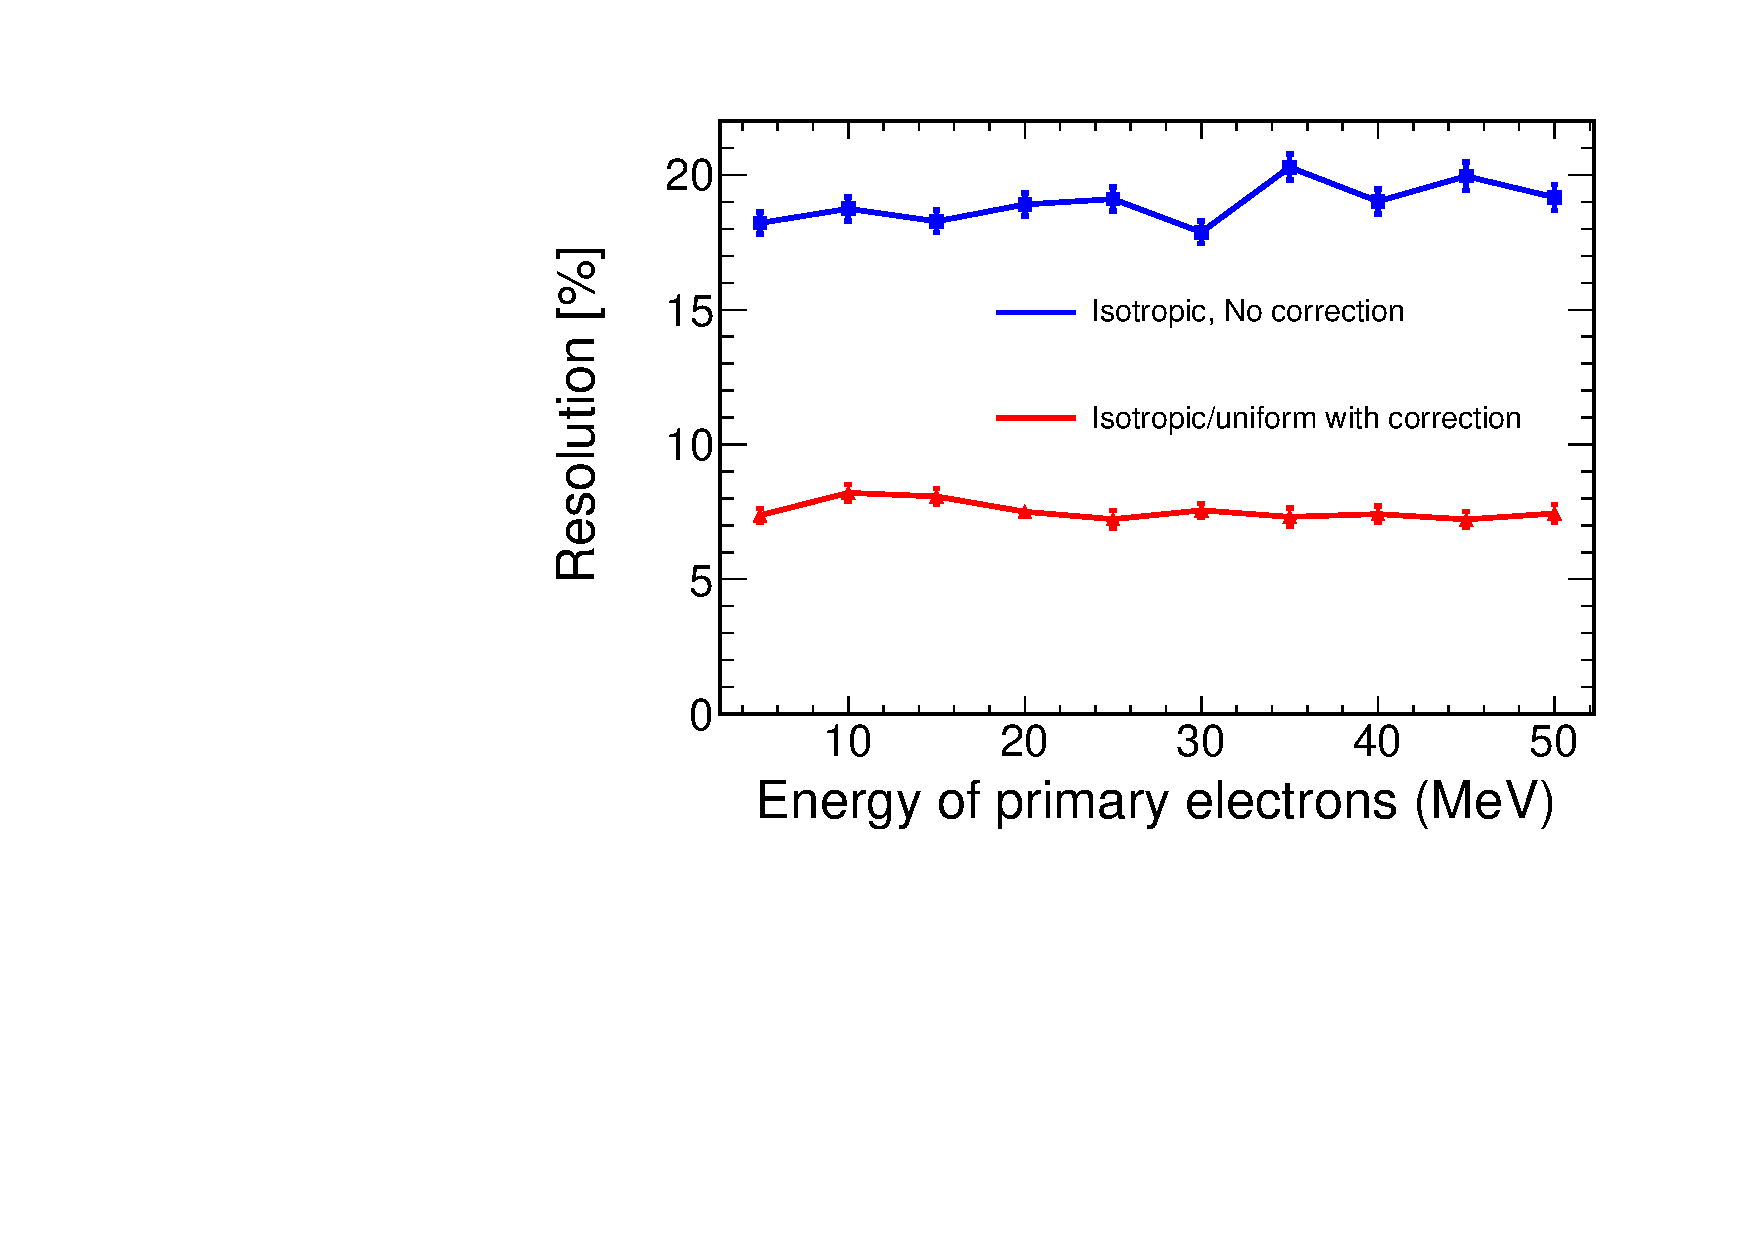
\includegraphics[width=0.45\textwidth]{correction.pdf} 
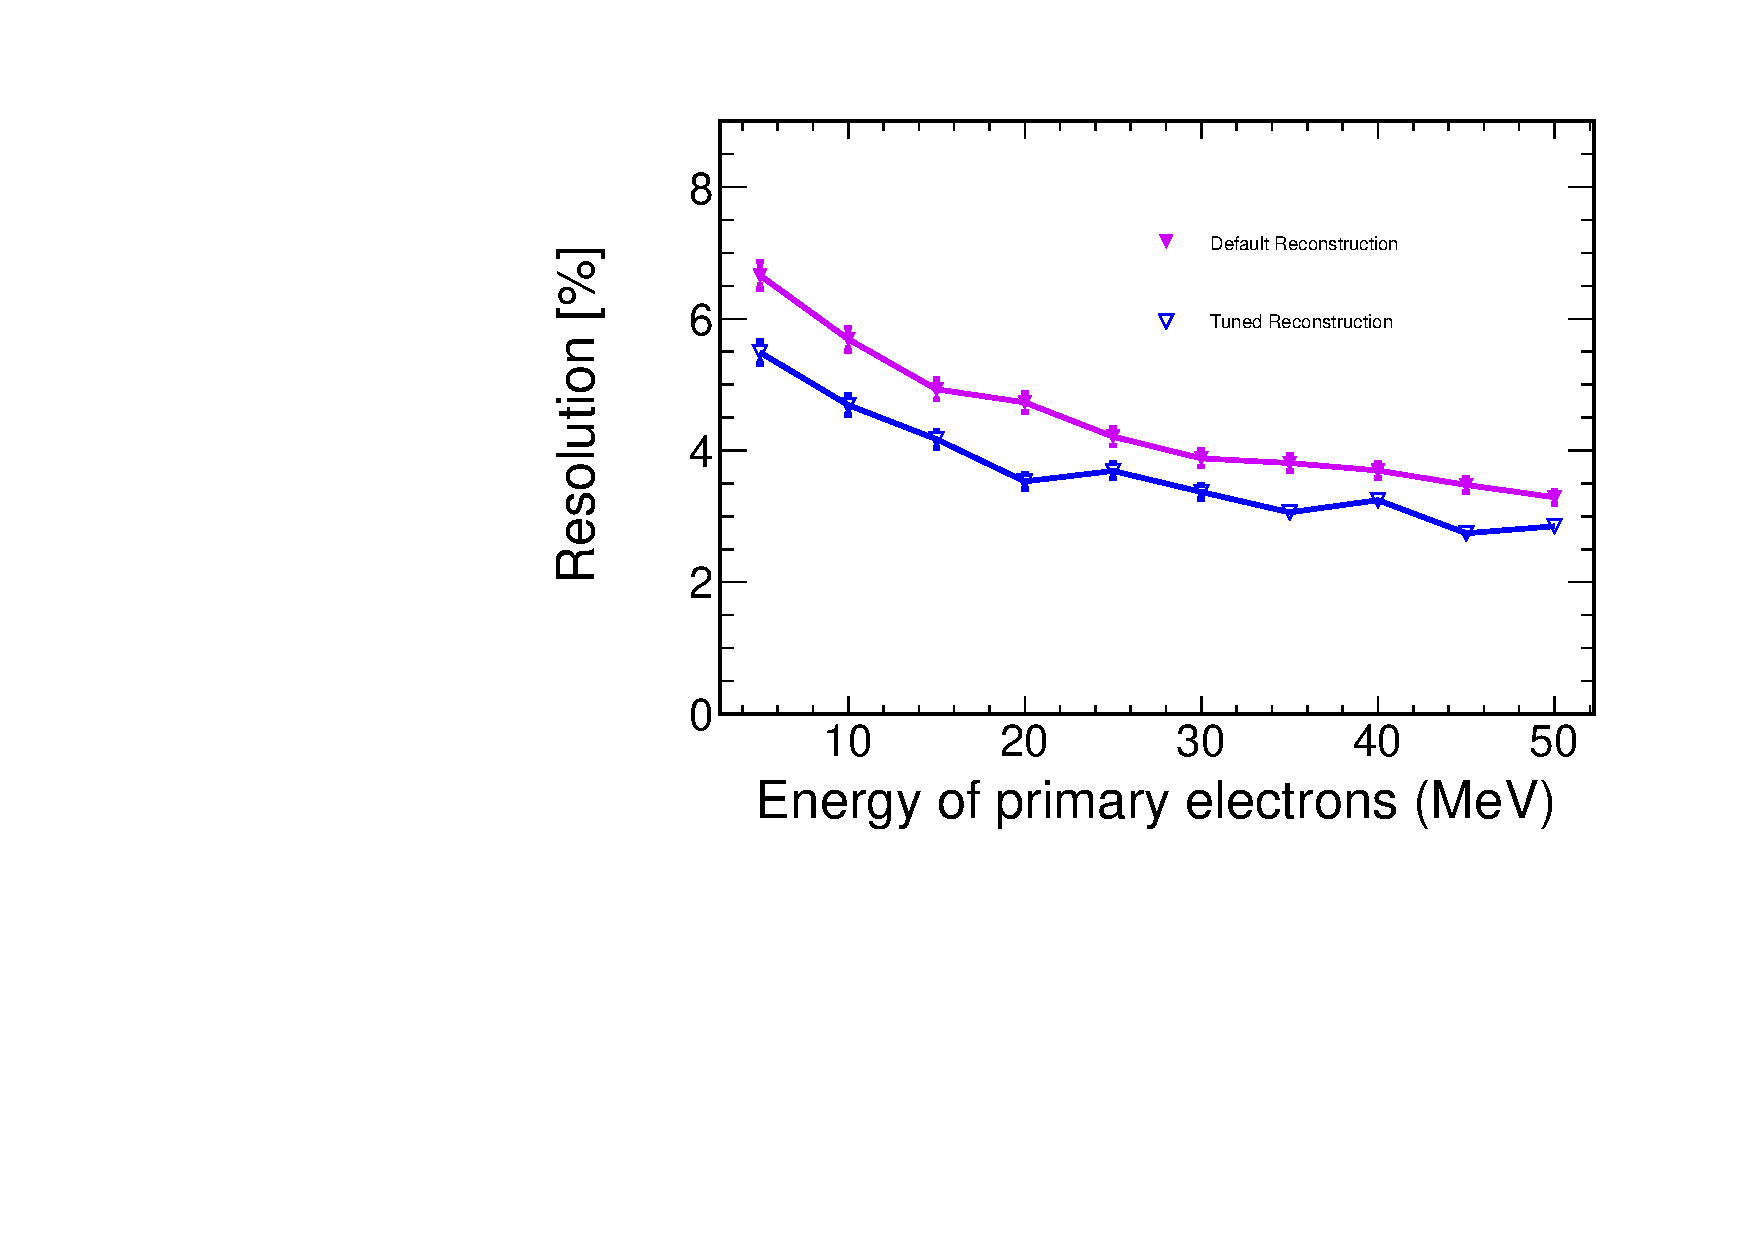
\includegraphics[width=0.45\textwidth]{hitfinder.pdf} 
 \caption[Comparisons of energy resolution]{Left: Comparison of energy
   resolution (defined as $\sigma/E$, where $\sigma$ is the spread of
   the collection-plane-charge-based event energy $E$ for a
   monoenergetic electron), with and without electron-lifetime
   correction, as a function of electron energy (assumptions: 3~ms
   drift time, 1.63~mm/$\mu$s drift velocity, and 2.5~m maximum drift
   length). The blue curve is the energy resolution of isotropic and
   uniform electrons without electron-lifetime correction. The red
   curve is the energy resolution with electron-lifetime correction
   based on MC truth.  Right: Comparison of energy resolution before
   and after tuning the reconstruction algorithm (for fixed
   position/direction electron events).}\label{fig:lowe_res}
\end{figure}

Also under study is the potential for tagging $\nu_e$CC absorption
events ($\nu_e +{}^{40}{\rm Ar} \rightarrow e^- +{}^{40}{\rm K^*}$)
using the cascade of de-excitation $\gamma$ rays (that Compton-scatter
in the detector); this should serve the dual purposes of rejecting
background and isolating the CC component of the supernova burst
signal.  Reconstructing these gammas also improves the neutrino energy
measurement.





